\documentclass[]{article}
\usepackage{lmodern}
\usepackage{amssymb,amsmath}
\usepackage{ifxetex,ifluatex}
\usepackage{fixltx2e} % provides \textsubscript
\ifnum 0\ifxetex 1\fi\ifluatex 1\fi=0 % if pdftex
  \usepackage[T1]{fontenc}
  \usepackage[utf8]{inputenc}
\else % if luatex or xelatex
  \ifxetex
    \usepackage{mathspec}
  \else
    \usepackage{fontspec}
  \fi
  \defaultfontfeatures{Ligatures=TeX,Scale=MatchLowercase}
\fi
% use upquote if available, for straight quotes in verbatim environments
\IfFileExists{upquote.sty}{\usepackage{upquote}}{}
% use microtype if available
\IfFileExists{microtype.sty}{%
\usepackage{microtype}
\UseMicrotypeSet[protrusion]{basicmath} % disable protrusion for tt fonts
}{}
\usepackage[margin=1in]{geometry}
\usepackage{hyperref}
\hypersetup{unicode=true,
            pdftitle={WorMotel Heritability with activity levels},
            pdfauthor={Tim C.},
            pdfborder={0 0 0},
            breaklinks=true}
\urlstyle{same}  % don't use monospace font for urls
\usepackage{color}
\usepackage{fancyvrb}
\newcommand{\VerbBar}{|}
\newcommand{\VERB}{\Verb[commandchars=\\\{\}]}
\DefineVerbatimEnvironment{Highlighting}{Verbatim}{commandchars=\\\{\}}
% Add ',fontsize=\small' for more characters per line
\usepackage{framed}
\definecolor{shadecolor}{RGB}{248,248,248}
\newenvironment{Shaded}{\begin{snugshade}}{\end{snugshade}}
\newcommand{\AlertTok}[1]{\textcolor[rgb]{0.94,0.16,0.16}{#1}}
\newcommand{\AnnotationTok}[1]{\textcolor[rgb]{0.56,0.35,0.01}{\textbf{\textit{#1}}}}
\newcommand{\AttributeTok}[1]{\textcolor[rgb]{0.77,0.63,0.00}{#1}}
\newcommand{\BaseNTok}[1]{\textcolor[rgb]{0.00,0.00,0.81}{#1}}
\newcommand{\BuiltInTok}[1]{#1}
\newcommand{\CharTok}[1]{\textcolor[rgb]{0.31,0.60,0.02}{#1}}
\newcommand{\CommentTok}[1]{\textcolor[rgb]{0.56,0.35,0.01}{\textit{#1}}}
\newcommand{\CommentVarTok}[1]{\textcolor[rgb]{0.56,0.35,0.01}{\textbf{\textit{#1}}}}
\newcommand{\ConstantTok}[1]{\textcolor[rgb]{0.00,0.00,0.00}{#1}}
\newcommand{\ControlFlowTok}[1]{\textcolor[rgb]{0.13,0.29,0.53}{\textbf{#1}}}
\newcommand{\DataTypeTok}[1]{\textcolor[rgb]{0.13,0.29,0.53}{#1}}
\newcommand{\DecValTok}[1]{\textcolor[rgb]{0.00,0.00,0.81}{#1}}
\newcommand{\DocumentationTok}[1]{\textcolor[rgb]{0.56,0.35,0.01}{\textbf{\textit{#1}}}}
\newcommand{\ErrorTok}[1]{\textcolor[rgb]{0.64,0.00,0.00}{\textbf{#1}}}
\newcommand{\ExtensionTok}[1]{#1}
\newcommand{\FloatTok}[1]{\textcolor[rgb]{0.00,0.00,0.81}{#1}}
\newcommand{\FunctionTok}[1]{\textcolor[rgb]{0.00,0.00,0.00}{#1}}
\newcommand{\ImportTok}[1]{#1}
\newcommand{\InformationTok}[1]{\textcolor[rgb]{0.56,0.35,0.01}{\textbf{\textit{#1}}}}
\newcommand{\KeywordTok}[1]{\textcolor[rgb]{0.13,0.29,0.53}{\textbf{#1}}}
\newcommand{\NormalTok}[1]{#1}
\newcommand{\OperatorTok}[1]{\textcolor[rgb]{0.81,0.36,0.00}{\textbf{#1}}}
\newcommand{\OtherTok}[1]{\textcolor[rgb]{0.56,0.35,0.01}{#1}}
\newcommand{\PreprocessorTok}[1]{\textcolor[rgb]{0.56,0.35,0.01}{\textit{#1}}}
\newcommand{\RegionMarkerTok}[1]{#1}
\newcommand{\SpecialCharTok}[1]{\textcolor[rgb]{0.00,0.00,0.00}{#1}}
\newcommand{\SpecialStringTok}[1]{\textcolor[rgb]{0.31,0.60,0.02}{#1}}
\newcommand{\StringTok}[1]{\textcolor[rgb]{0.31,0.60,0.02}{#1}}
\newcommand{\VariableTok}[1]{\textcolor[rgb]{0.00,0.00,0.00}{#1}}
\newcommand{\VerbatimStringTok}[1]{\textcolor[rgb]{0.31,0.60,0.02}{#1}}
\newcommand{\WarningTok}[1]{\textcolor[rgb]{0.56,0.35,0.01}{\textbf{\textit{#1}}}}
\usepackage{graphicx,grffile}
\makeatletter
\def\maxwidth{\ifdim\Gin@nat@width>\linewidth\linewidth\else\Gin@nat@width\fi}
\def\maxheight{\ifdim\Gin@nat@height>\textheight\textheight\else\Gin@nat@height\fi}
\makeatother
% Scale images if necessary, so that they will not overflow the page
% margins by default, and it is still possible to overwrite the defaults
% using explicit options in \includegraphics[width, height, ...]{}
\setkeys{Gin}{width=\maxwidth,height=\maxheight,keepaspectratio}
\IfFileExists{parskip.sty}{%
\usepackage{parskip}
}{% else
\setlength{\parindent}{0pt}
\setlength{\parskip}{6pt plus 2pt minus 1pt}
}
\setlength{\emergencystretch}{3em}  % prevent overfull lines
\providecommand{\tightlist}{%
  \setlength{\itemsep}{0pt}\setlength{\parskip}{0pt}}
\setcounter{secnumdepth}{0}
% Redefines (sub)paragraphs to behave more like sections
\ifx\paragraph\undefined\else
\let\oldparagraph\paragraph
\renewcommand{\paragraph}[1]{\oldparagraph{#1}\mbox{}}
\fi
\ifx\subparagraph\undefined\else
\let\oldsubparagraph\subparagraph
\renewcommand{\subparagraph}[1]{\oldsubparagraph{#1}\mbox{}}
\fi

%%% Use protect on footnotes to avoid problems with footnotes in titles
\let\rmarkdownfootnote\footnote%
\def\footnote{\protect\rmarkdownfootnote}

%%% Change title format to be more compact
\usepackage{titling}

% Create subtitle command for use in maketitle
\newcommand{\subtitle}[1]{
  \posttitle{
    \begin{center}\large#1\end{center}
    }
}

\setlength{\droptitle}{-2em}
  \title{WorMotel Heritability with activity levels}
  \pretitle{\vspace{\droptitle}\centering\huge}
  \posttitle{\par}
  \author{Tim C.}
  \preauthor{\centering\large\emph}
  \postauthor{\par}
  \predate{\centering\large\emph}
  \postdate{\par}
  \date{1/19/2018}


\begin{document}
\maketitle

This code uses processed survival data from Chris Fang-Yen's lab to
calcualte heritability of survival traits. The data were collected with
WorMotel in winter 2017 by Matt Churgin at UPenn.

\hypertarget{read-in-data-and-define-functions}{%
\paragraph{Read in data and define
functions}\label{read-in-data-and-define-functions}}

\begin{Shaded}
\begin{Highlighting}[]
\NormalTok{df <-}\StringTok{ }\KeywordTok{as.data.frame}\NormalTok{(}\KeywordTok{read.csv}\NormalTok{(}\DataTypeTok{file =} \StringTok{"20170116_FullProcessed.csv"}\NormalTok{, }\DataTypeTok{header =}\NormalTok{ T))}

\KeywordTok{glimpse}\NormalTok{(df)}
\end{Highlighting}
\end{Shaded}

\begin{verbatim}
## Observations: 64,800
## Variables: 8
## $ strain        <fct> CB4856, CB4856, CB4856, CB4856, CB4856, CB4856, ...
## $ tech_rep      <int> 2, 2, 2, 2, 2, 2, 2, 2, 2, 2, 2, 2, 2, 2, 2, 2, ...
## $ bio_rep       <int> 1, 1, 1, 1, 1, 1, 1, 1, 1, 1, 1, 1, 1, 1, 1, 1, ...
## $ rep           <int> 1, 1, 1, 1, 1, 1, 1, 1, 1, 1, 1, 1, 1, 1, 1, 1, ...
## $ life_span     <dbl> NA, NA, NA, NA, NA, NA, NA, NA, NA, NA, NA, NA, ...
## $ activity_type <fct> stim, stim, stim, stim, stim, stim, stim, stim, ...
## $ time_d        <dbl> 1.5, 3.0, 4.5, 6.0, 8.0, 9.5, 11.5, 13.0, 15.0, ...
## $ activity      <int> 0, 0, 0, 0, 0, 0, 0, 0, 0, 0, 0, 0, 0, 0, 0, 0, ...
\end{verbatim}

\begin{Shaded}
\begin{Highlighting}[]
\CommentTok{# define heritability test}
\NormalTok{H2.test <-}\StringTok{ }\ControlFlowTok{function}\NormalTok{(data)\{}
  
\NormalTok{  pheno <-}\StringTok{ }\KeywordTok{as.data.frame}\NormalTok{(dplyr}\OperatorTok{::}\KeywordTok{select}\NormalTok{(data, phenotype))[,}\DecValTok{1}\NormalTok{]}
\NormalTok{  strain <-}\StringTok{ }\KeywordTok{as.factor}\NormalTok{(data}\OperatorTok{$}\NormalTok{strain)}
  
\NormalTok{  reffMod <-}\StringTok{ }\NormalTok{lme4}\OperatorTok{::}\KeywordTok{lmer}\NormalTok{(pheno }\OperatorTok{~}\StringTok{ }\DecValTok{1} \OperatorTok{+}\StringTok{ }\NormalTok{(}\DecValTok{1}\OperatorTok{|}\NormalTok{strain))}
  
\NormalTok{  Variances <-}\StringTok{ }\KeywordTok{as.data.frame}\NormalTok{(lme4}\OperatorTok{::}\KeywordTok{VarCorr}\NormalTok{(reffMod, }\DataTypeTok{comp =} \StringTok{"Variance"}\NormalTok{))}
  
\NormalTok{  Vg <-}\StringTok{ }\NormalTok{Variances}\OperatorTok{$}\NormalTok{vcov[}\DecValTok{1}\NormalTok{]}
\NormalTok{  Ve <-}\StringTok{ }\NormalTok{Variances}\OperatorTok{$}\NormalTok{vcov[}\DecValTok{2}\NormalTok{]}
\NormalTok{  H2 <-}\StringTok{ }\NormalTok{Vg}\OperatorTok{/}\NormalTok{(Vg}\OperatorTok{+}\NormalTok{Ve)}
  
  \KeywordTok{return}\NormalTok{(H2)}
\NormalTok{\}}

\CommentTok{# remove outliers function}
\NormalTok{remove_outliers <-}\StringTok{ }\ControlFlowTok{function}\NormalTok{(x, }\DataTypeTok{na.rm =} \OtherTok{TRUE}\NormalTok{, ...) \{}
\NormalTok{  qnt <-}\StringTok{ }\KeywordTok{quantile}\NormalTok{(x, }\DataTypeTok{probs=}\KeywordTok{c}\NormalTok{(.}\DecValTok{25}\NormalTok{, }\FloatTok{.75}\NormalTok{), }\DataTypeTok{na.rm =}\NormalTok{ na.rm, ...)}
\NormalTok{  H <-}\StringTok{ }\FloatTok{1.5} \OperatorTok{*}\StringTok{ }\KeywordTok{IQR}\NormalTok{(x, }\DataTypeTok{na.rm =}\NormalTok{ na.rm)}
\NormalTok{  y <-}\StringTok{ }\NormalTok{x}
\NormalTok{  y[x }\OperatorTok{<}\StringTok{ }\NormalTok{(qnt[}\DecValTok{1}\NormalTok{] }\OperatorTok{-}\StringTok{ }\NormalTok{H)] <-}\StringTok{ }\OtherTok{NA}
\NormalTok{  y[x }\OperatorTok{>}\StringTok{ }\NormalTok{(qnt[}\DecValTok{2}\NormalTok{] }\OperatorTok{+}\StringTok{ }\NormalTok{H)] <-}\StringTok{ }\OtherTok{NA}
\NormalTok{  y}
\NormalTok{\}}
\end{Highlighting}
\end{Shaded}

 Each bio\_rep is treated as a block for the following analysis.
Technical replicates are ignored.

\#\#\#ANALYSIS 1: Focus on activity levels within block 1 across all
timepoints

\begin{verbatim}
## Warning: Removed 13 rows containing non-finite values (stat_boxplot).
\end{verbatim}

\begin{verbatim}
## Warning: Removed 251 rows containing missing values (geom_point).
\end{verbatim}

\includegraphics{20180119_ActivityHeritability_files/figure-latex/unnamed-chunk-3-1.pdf}
JU775 appears to retain higher activity levels compared to other strains
at later timepoints. I'm concerned about calculating heritability for
these timepoints however because the number of nematodes observed is 1
for some strains at day 19 and day 22. I'll do the calculation anyway
and see what we get.

\hypertarget{heritability-for-activity-levels-at-different-timepoints-within-block-1}{%
\paragraph{Heritability for activity levels at different timepoints
within block
1}\label{heritability-for-activity-levels-at-different-timepoints-within-block-1}}

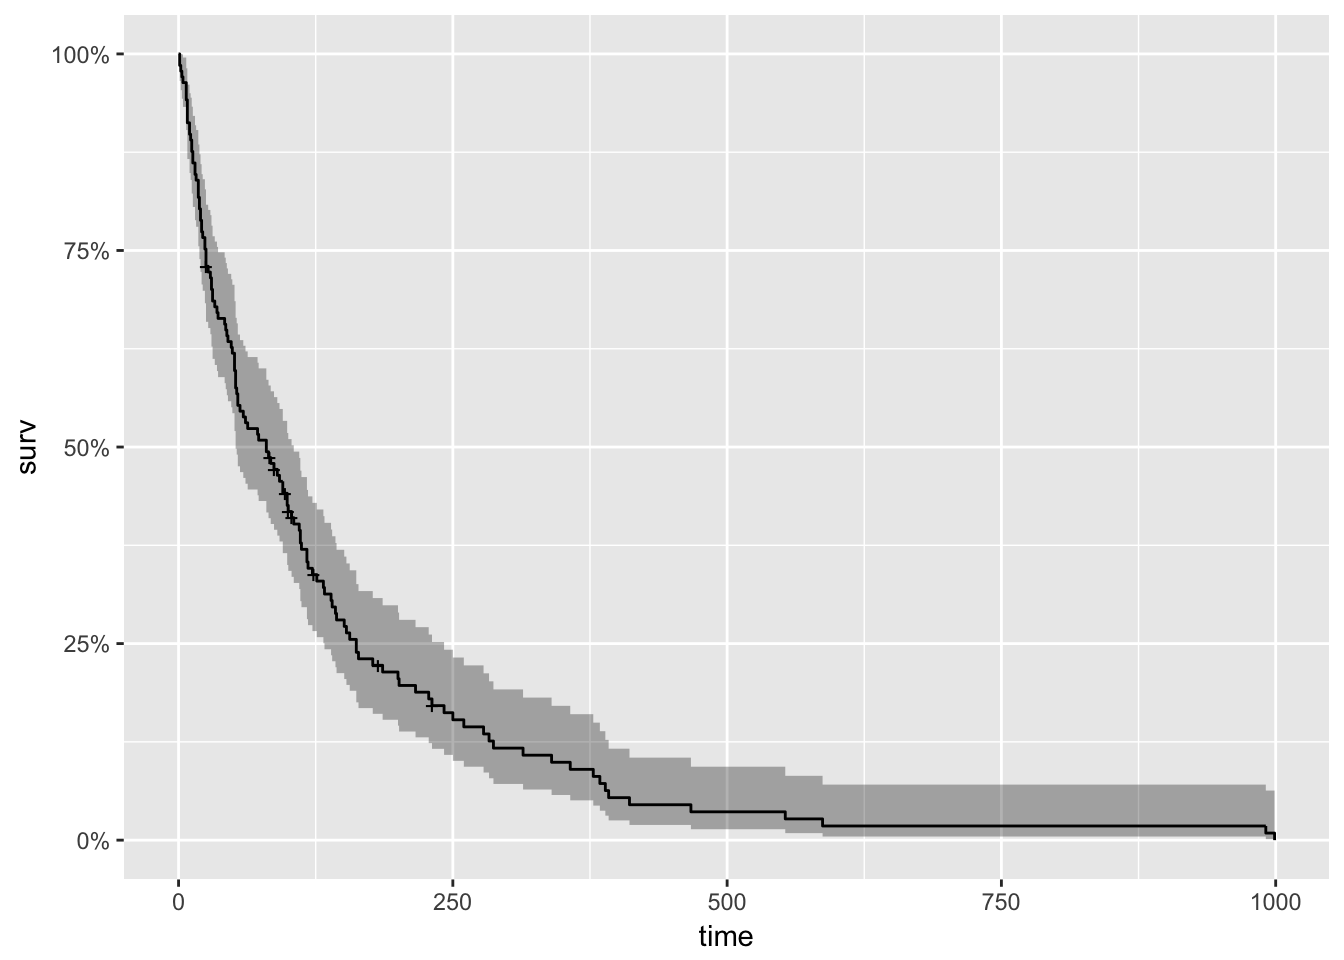
\includegraphics{20180119_ActivityHeritability_files/figure-latex/unnamed-chunk-4-1.pdf}
We see very high heritability for activity traits at later timepoints.
However, we have less than two replicates for some strains at the later
time points. I'll try filtering timepoints to those containing at least
5 reps per strain.

\hypertarget{recalculate-heritability-on-timepoints-with-at-least-5-reps-per-strain}{%
\paragraph{Recalculate heritability on timepoints with at least 5 reps
per
strain}\label{recalculate-heritability-on-timepoints-with-at-least-5-reps-per-strain}}

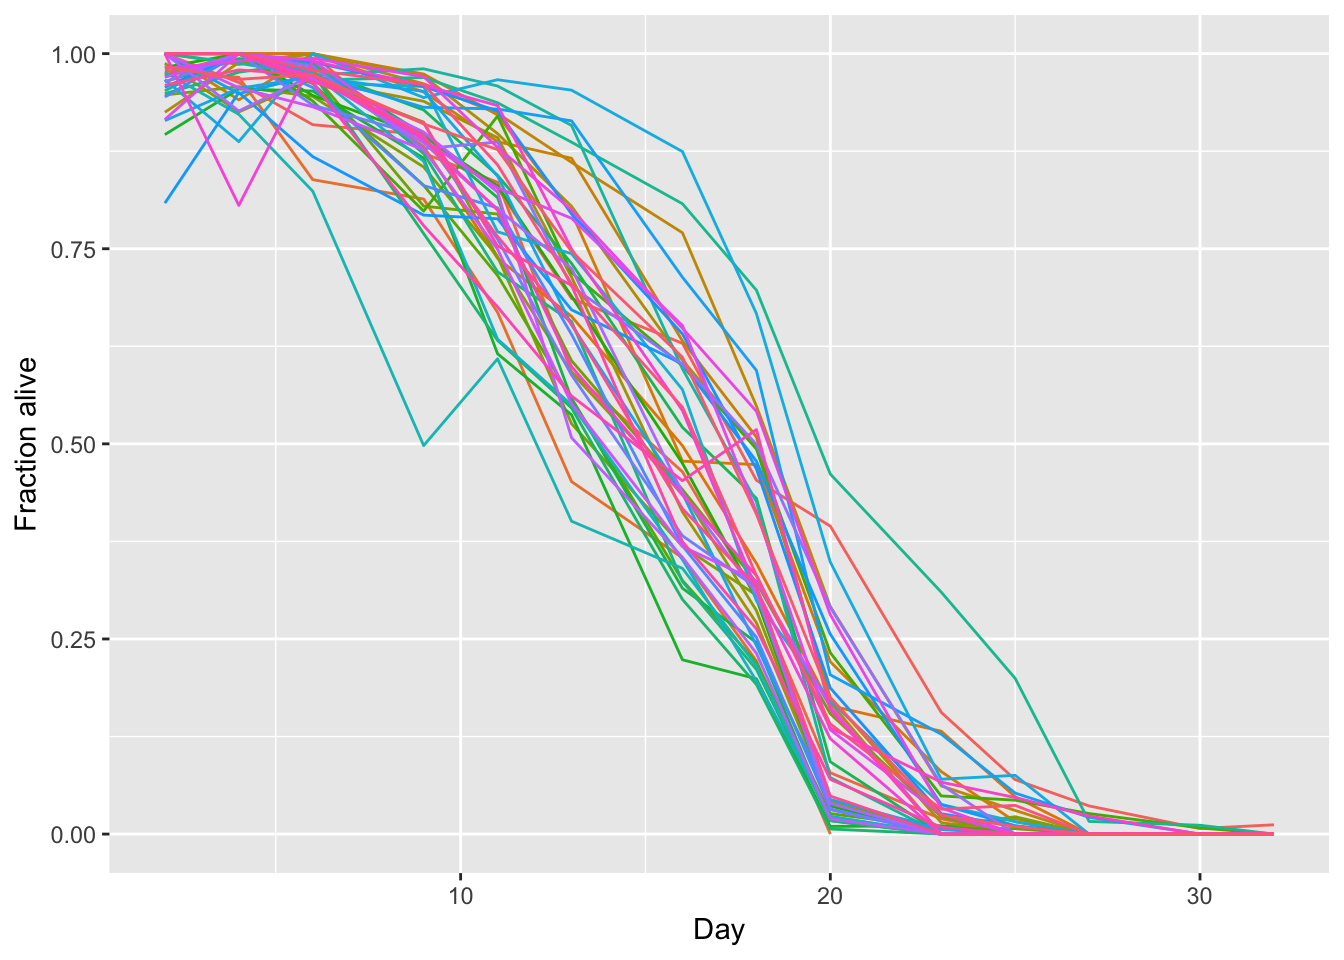
\includegraphics{20180119_ActivityHeritability_files/figure-latex/unnamed-chunk-5-1.pdf}
Heritability is still high for activity traits at 17 days. Below is a
more detailed plot of those timepoints.

\#\#\#\#Heritability for time points with at lest 5 reps per strain

\begin{verbatim}
## Warning: Removed 80 rows containing missing values (geom_point).
\end{verbatim}

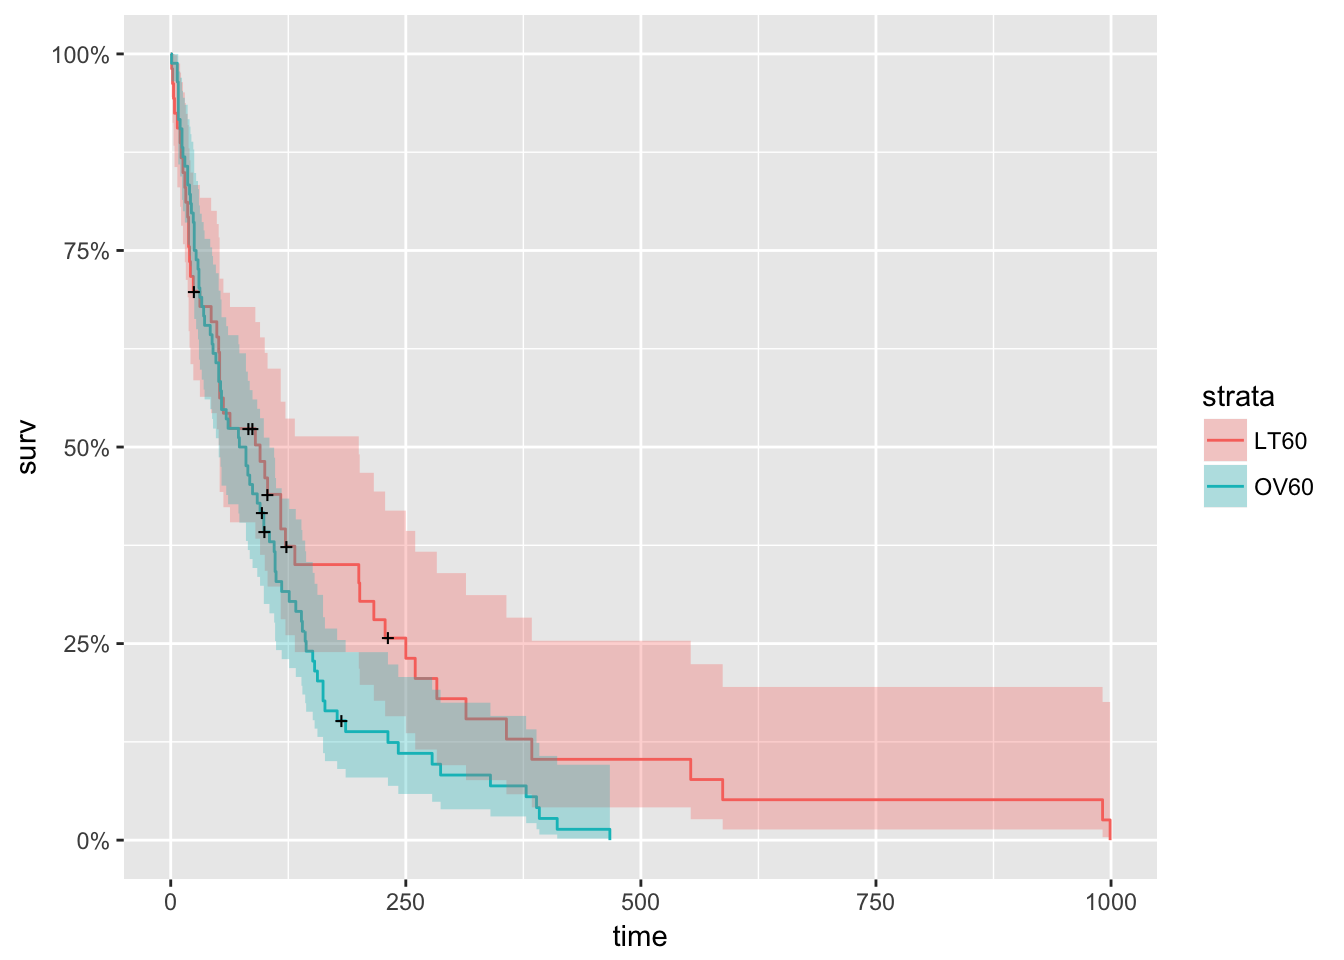
\includegraphics{20180119_ActivityHeritability_files/figure-latex/unnamed-chunk-6-1.pdf}

\#\#\#ANALYSIS 1 CONCLUSIONS: 1) Heritability for both stim and base
activity traits at day 17 exceeds the 0.2 threshold (Fig. 3). 2) The
JU775 strain is likely driving heritability in activity traits since it
maintains much higher activity levels at late timepoints (Fig. 4). 3)
The difference between stimulated and base activity is small for most
individuals (Figs. 1, 4). Is this expected?

\#\#\#ANALYSIS 2: Fit model to the drop in activity levels over time and
calculate heritability on model parameters. For now I'm moving on to
fitting a curve to the decrease in activity levels over time. We might
see high heritability in fit parameters. Outlier activity levels are
filtered for this analysis.

\begin{verbatim}
## `geom_smooth()` using method = 'loess'
\end{verbatim}

\begin{verbatim}
## Warning: Removed 1540 rows containing non-finite values (stat_smooth).
\end{verbatim}

\begin{verbatim}
## Warning: Removed 1540 rows containing missing values (geom_point).
\end{verbatim}

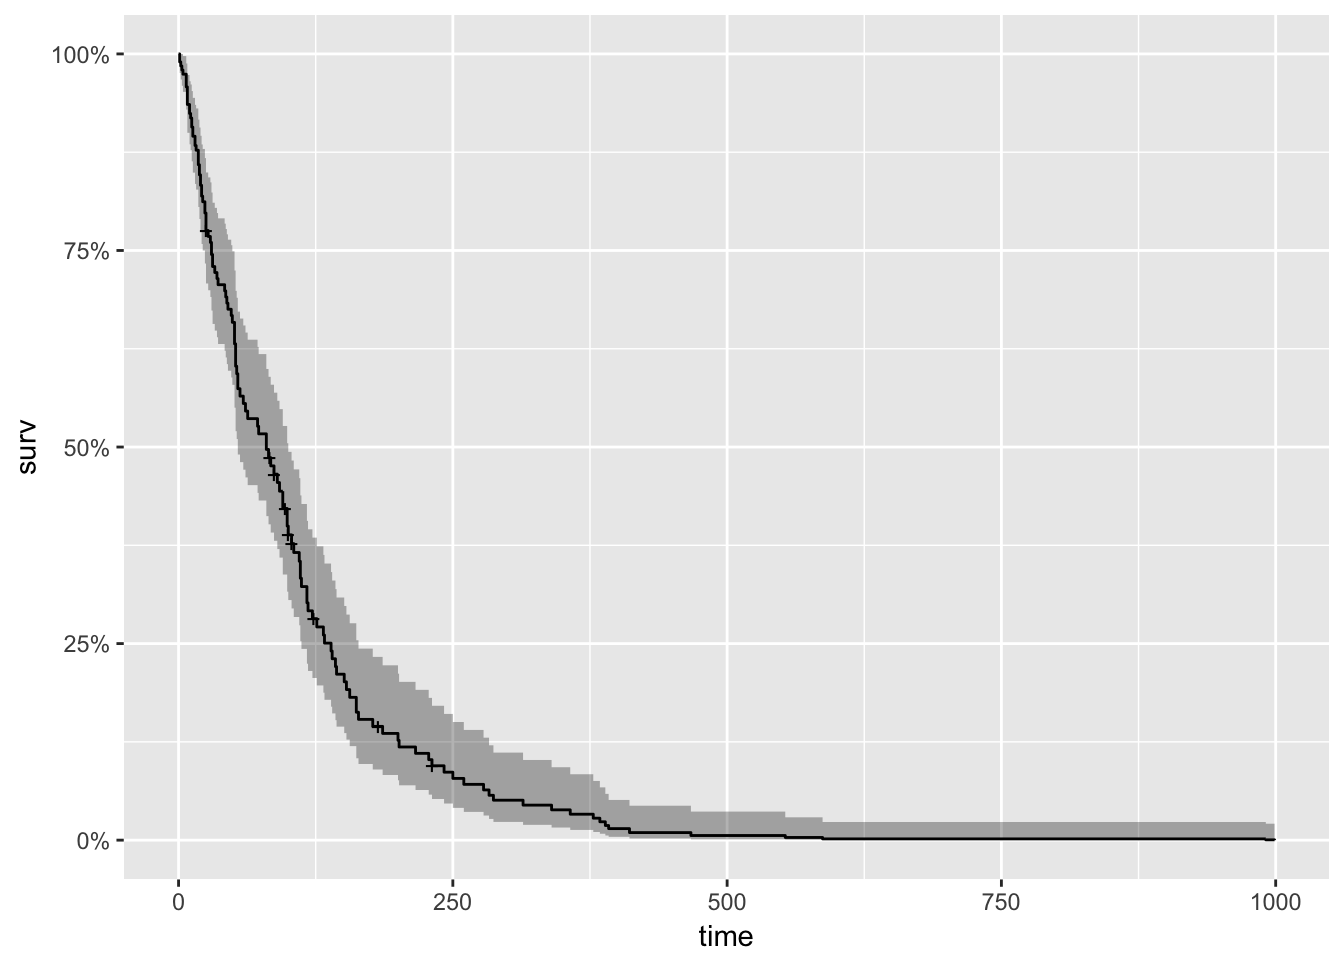
\includegraphics{20180119_ActivityHeritability_files/figure-latex/unnamed-chunk-7-1.pdf}
It looks like we may be able to fit curves to the acivity data, but it
is noisy. The Loess fit looks similar to a Ricker function with an early
hump and then exponential decay. Stim and base traits looks the most
promising. Ricker function, f(x) = a\emph{x}exp(1)\^{}(b*x).

\hypertarget{testing-fit-of-ricker-function-to-cb4856-data-for-each-block}{%
\paragraph{Testing fit of Ricker function to CB4856 data for each
block}\label{testing-fit-of-ricker-function-to-cb4856-data-for-each-block}}

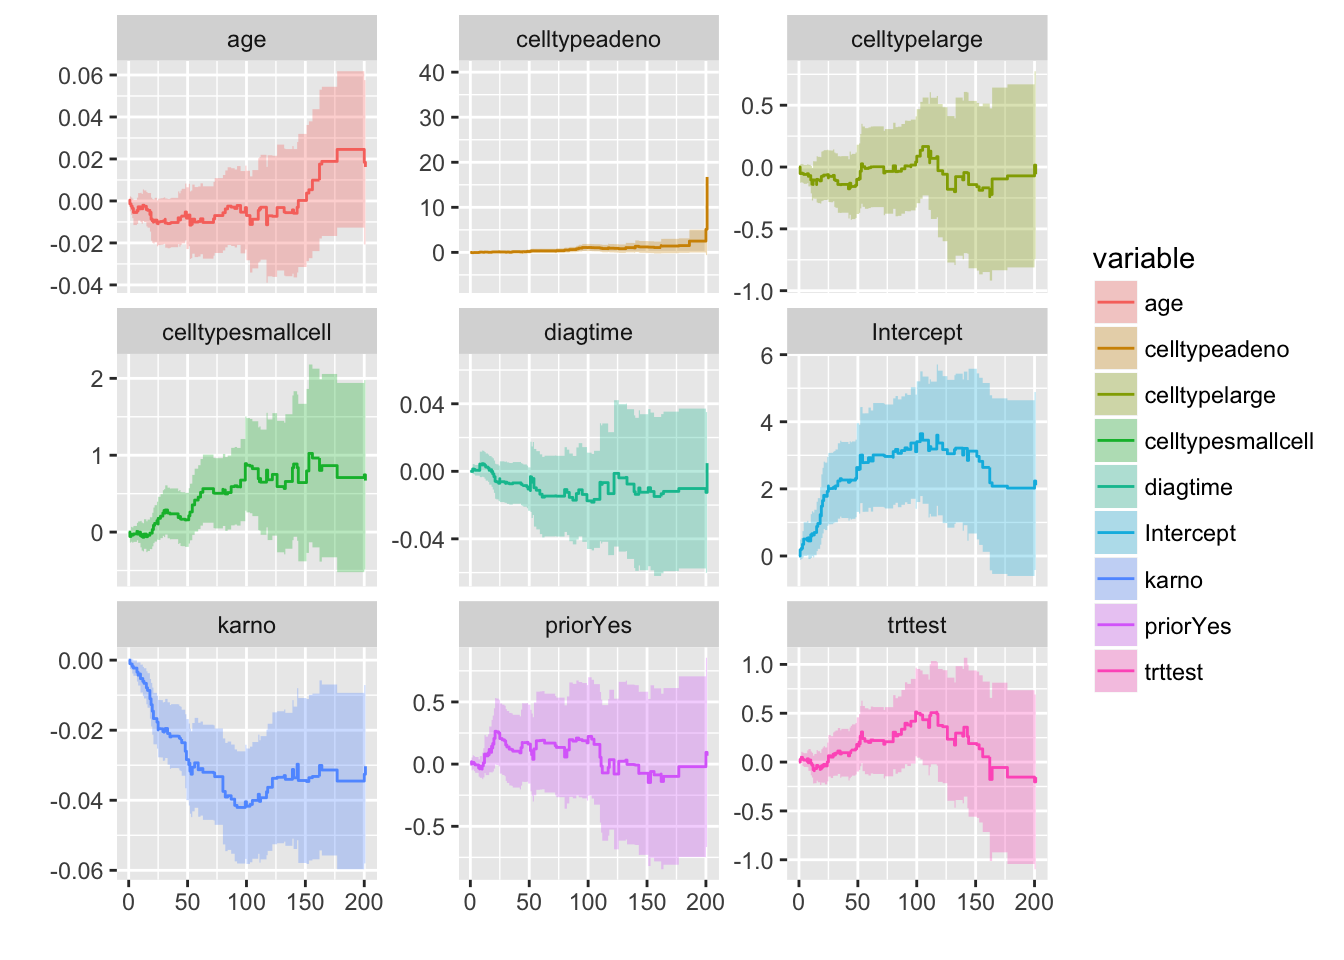
\includegraphics{20180119_ActivityHeritability_files/figure-latex/unnamed-chunk-8-1.pdf}
Ricker model looks similar to loess fit for blocks 1-3. However, the
shape of the fit is very different among the blocks. I'll extract
\texttt{a} and \texttt{b} parameters from Ricker f(x) =
a\emph{x}exp(1)\^{}(b*x) for each strain and each block then calculate
heritability.

\#\#\#\#Plotting raw Ricker fit parameters (a) and (b) for stim activity
and base activity
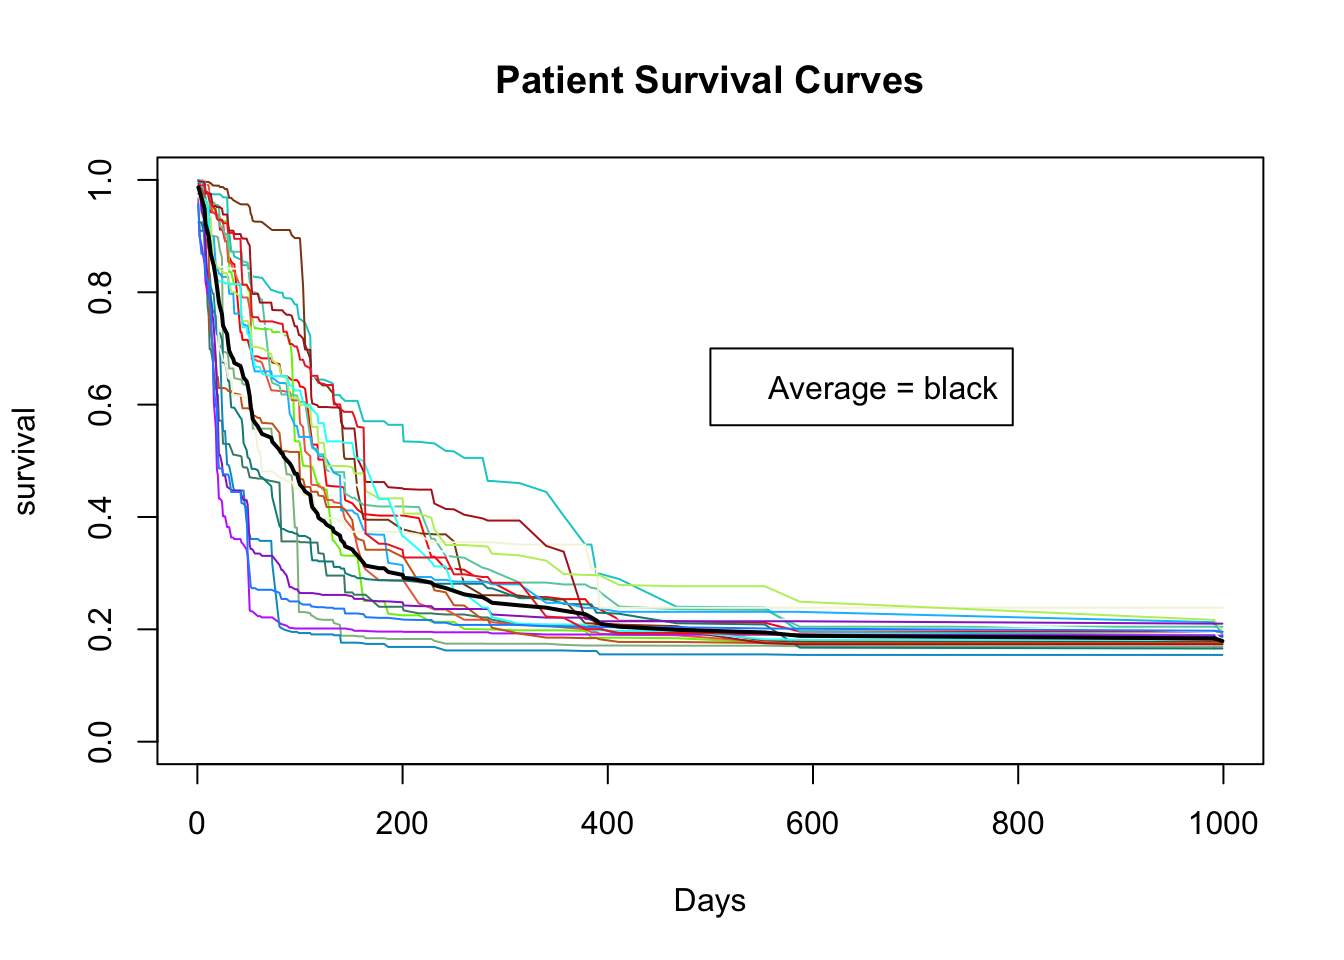
\includegraphics{20180119_ActivityHeritability_files/figure-latex/unnamed-chunk-9-1.pdf}
Huge outliers coming from misfit model, mostly in block 6. I can filter
these outlier parameter estimates and replot.

\hypertarget{ricker-fit-parameters-with-outliers-removed}{%
\paragraph{Ricker fit parameters with outliers
removed}\label{ricker-fit-parameters-with-outliers-removed}}

\begin{verbatim}
## Warning: Removed 37 rows containing non-finite values (stat_boxplot).
\end{verbatim}

\begin{verbatim}
## Warning: Removed 37 rows containing missing values (geom_point).
\end{verbatim}

\includegraphics{20180119_ActivityHeritability_files/figure-latex/unnamed-chunk-10-1.pdf}
Outlier filtered data looks better. I'll calculate heritability with
outlier filtered and block effect corrected data.

\#\#\#\#Correct for block effect and plot residuals

\begin{Shaded}
\begin{Highlighting}[]
\CommentTok{# Process data for heritability calculation}
\NormalTok{new_df <-}\StringTok{ }\NormalTok{df_proc }\OperatorTok
\StringTok{  }\NormalTok{tidyr}\OperatorTok{::}\KeywordTok{gather}\NormalTok{(trait, phenotype, }\OperatorTok{-}\NormalTok{block, }\OperatorTok{-}\NormalTok{strain, }\OperatorTok{-}\NormalTok{rep, }\OperatorTok{-}\NormalTok{time_d) }\OperatorTok
\StringTok{  }\NormalTok{dplyr}\OperatorTok{::}\KeywordTok{filter}\NormalTok{(trait }\OperatorTok\StringTok{ }\KeywordTok{c}\NormalTok{(}\StringTok{"base"}\NormalTok{, }\StringTok{"stim"}\NormalTok{)) }\OperatorTok
\StringTok{  }\NormalTok{dplyr}\OperatorTok{::}\KeywordTok{group_by}\NormalTok{(block, strain, trait) }\OperatorTok
\StringTok{  }\NormalTok{dplyr}\OperatorTok{::}\KeywordTok{do}\NormalTok{(}\KeywordTok{tidy}\NormalTok{(}\KeywordTok{nlsLM}\NormalTok{(phenotype }\OperatorTok{~}\StringTok{ }\NormalTok{a}\OperatorTok{*}\NormalTok{time_d}\OperatorTok{*}\KeywordTok{exp}\NormalTok{(}\DecValTok{1}\NormalTok{)}\OperatorTok{^}\NormalTok{(b}\OperatorTok{*}\NormalTok{time_d),}
                    \DataTypeTok{data =}\NormalTok{ ., }\DataTypeTok{start =} \KeywordTok{list}\NormalTok{(}\DataTypeTok{a=}\DecValTok{100}\NormalTok{,}\DataTypeTok{b=}\FloatTok{0.2}\NormalTok{), }\DataTypeTok{control =} \KeywordTok{nls.lm.control}\NormalTok{(}\DataTypeTok{maxiter =} \DecValTok{200}\NormalTok{)))) }\OperatorTok\StringTok{ }\CommentTok{# Fit Ricker function to base activity and stim activity for each strain within each block}
\StringTok{  }\NormalTok{dplyr}\OperatorTok{::}\KeywordTok{ungroup}\NormalTok{() }\OperatorTok
\StringTok{  }\NormalTok{dplyr}\OperatorTok{::}\KeywordTok{group_by}\NormalTok{(trait, term) }\OperatorTok\StringTok{ }
\StringTok{  }\NormalTok{dplyr}\OperatorTok{::}\KeywordTok{mutate}\NormalTok{(}\DataTypeTok{phenotype =} \KeywordTok{remove_outliers}\NormalTok{(estimate)) }\OperatorTok\StringTok{ }\CommentTok{#identify and remove outliers}
\StringTok{  }\NormalTok{dplyr}\OperatorTok{::}\KeywordTok{ungroup}\NormalTok{() }\OperatorTok
\StringTok{  }\NormalTok{dplyr}\OperatorTok{::}\KeywordTok{filter}\NormalTok{(}\KeywordTok{complete.cases}\NormalTok{(.)) }\OperatorTok\StringTok{ }\CommentTok{# remove outlier rows from data frame}
\StringTok{  }\NormalTok{dplyr}\OperatorTok{::}\KeywordTok{group_by}\NormalTok{(trait, term) }\OperatorTok
\StringTok{  }\NormalTok{dplyr}\OperatorTok{::}\KeywordTok{mutate}\NormalTok{(}\DataTypeTok{phenotype =} \KeywordTok{residuals}\NormalTok{(}\KeywordTok{lm}\NormalTok{(estimate }\OperatorTok{~}\StringTok{ }\NormalTok{block)))  }\CommentTok{# regress out block effect}
  
\NormalTok{ricker <-}\StringTok{ }\KeywordTok{ggplot}\NormalTok{(new_df) }\OperatorTok{+}
\StringTok{  }\KeywordTok{aes}\NormalTok{(}\DataTypeTok{x =}\NormalTok{ strain, }\DataTypeTok{y =}\NormalTok{ phenotype) }\OperatorTok{+}
\StringTok{  }\KeywordTok{geom_boxplot}\NormalTok{(}\DataTypeTok{outlier.shape =} \OtherTok{NA}\NormalTok{) }\OperatorTok{+}
\StringTok{  }\KeywordTok{geom_jitter}\NormalTok{(}\KeywordTok{aes}\NormalTok{(}\DataTypeTok{color =} \KeywordTok{factor}\NormalTok{(block)), }\DataTypeTok{width =} \FloatTok{.25}\NormalTok{) }\OperatorTok{+}
\StringTok{  }\KeywordTok{facet_wrap}\NormalTok{(trait }\OperatorTok{~}\StringTok{ }\NormalTok{term, }\DataTypeTok{scales =} \StringTok{"free"}\NormalTok{) }\OperatorTok{+}
\StringTok{  }\KeywordTok{labs}\NormalTok{(}\DataTypeTok{title =} \StringTok{"FIGURE 9: Risidual ricker fit parameter estimates (outliers removed)"}\NormalTok{, }\DataTypeTok{y=}\StringTok{"residual parameter estimate"}\NormalTok{, }\DataTypeTok{x =} \StringTok{""}\NormalTok{, }\DataTypeTok{color =} \StringTok{"block"}\NormalTok{) }\OperatorTok{+}
\StringTok{  }\KeywordTok{theme_classic}\NormalTok{() }\OperatorTok{+}
\StringTok{  }\KeywordTok{theme}\NormalTok{(}\DataTypeTok{legend.position =} \StringTok{"right"}\NormalTok{)}
\NormalTok{ricker}
\end{Highlighting}
\end{Shaded}

\includegraphics{20180119_ActivityHeritability_files/figure-latex/unnamed-chunk-11-1.pdf}
Differences among strains is most pronounced for the stimulated activity
parameter \texttt{a} trait. The other traits do not appear to be as
different across strains.

\hypertarget{calculating-heritability-on-residual-ricker-fit-parameter-estimates-for-base-and-stimulated-activity}{%
\paragraph{Calculating heritability on residual Ricker fit parameter
estimates for base and stimulated
activity}\label{calculating-heritability-on-residual-ricker-fit-parameter-estimates-for-base-and-stimulated-activity}}

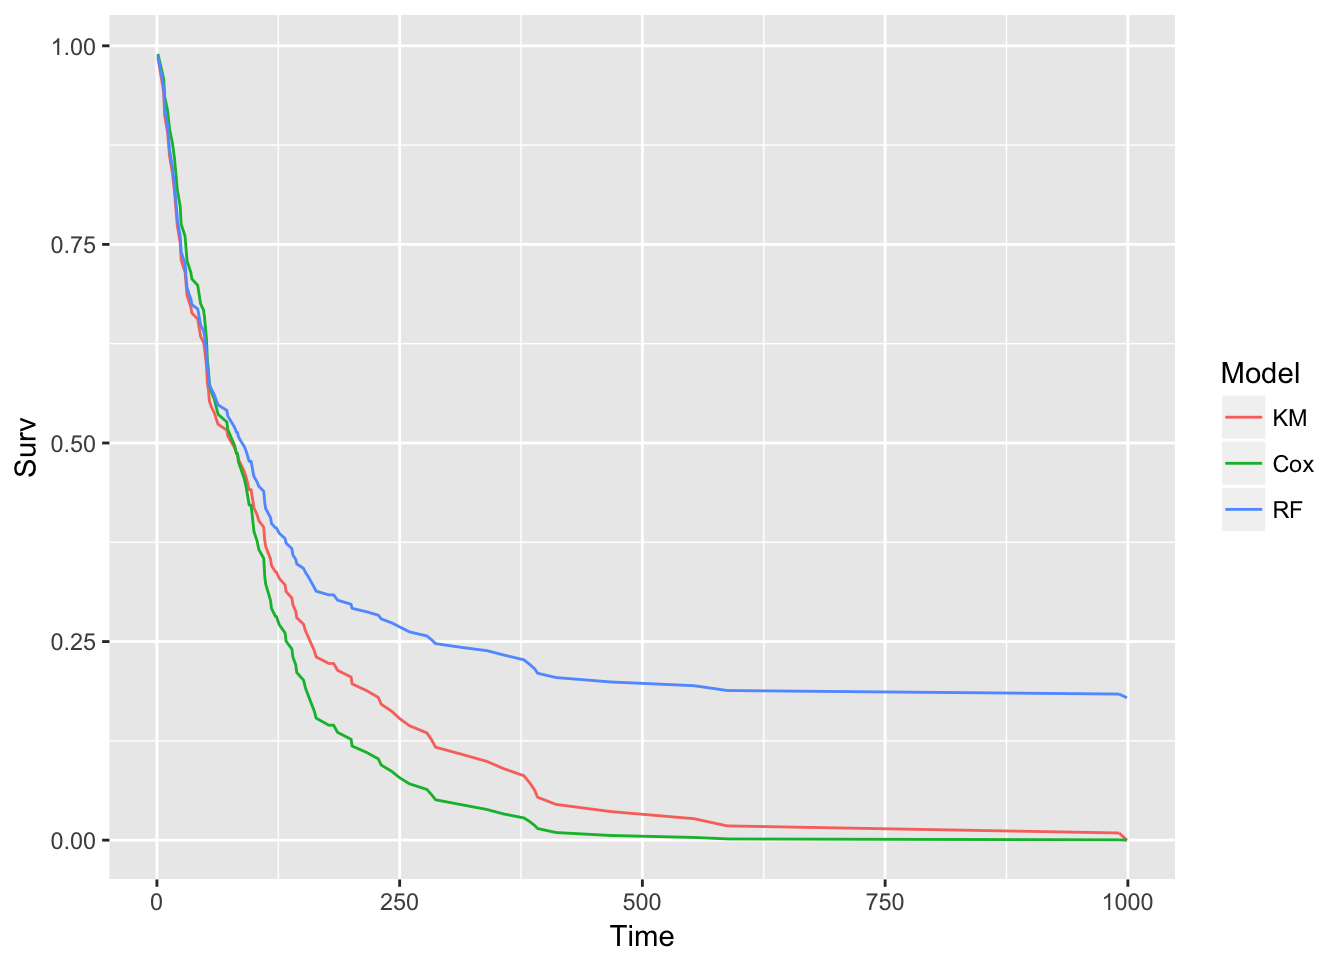
\includegraphics{20180119_ActivityHeritability_files/figure-latex/unnamed-chunk-12-1.pdf}

\hypertarget{analysis-2-conclusions}{%
\subsubsection{ANALYSIS 2 CONCLUSIONS:}\label{analysis-2-conclusions}}

 1) Ricker parameter estimates \texttt{a} and \texttt{b} are very
different among blocks even for the same strain (Fig. 6) 2) After
removing outliers and correcting for block effect, heritability is just
0.13 for the stim activity parameter \texttt{a} trait (Fig. 10).

\hypertarget{analysis-3-focus-on-day-15-activity-data-alone}{%
\subsubsection{ANALYSIS 3: Focus on day 15 activity data
alone}\label{analysis-3-focus-on-day-15-activity-data-alone}}

 I'm interested in day 15 data because 5 of the 6 blocks share this
timepoint and therefore we should have many replicates. The activity
traits below are taken from day 15 worms. Block 3 did not have a day 15
timepoint so it is excluded Base activity is the activity measure before
stimulus light. Stim activity is the activity level after stimulus light
was applied. stim - base activity is the difference between the two.

\hypertarget{plotting-individual-worm-activity-and-life-span-traits-for-day-15}{%
\paragraph{Plotting individual worm activity and life span traits for
day
15}\label{plotting-individual-worm-activity-and-life-span-traits-for-day-15}}

\includegraphics{20180119_ActivityHeritability_files/figure-latex/unnamed-chunk-13-1.pdf}
Block 2 has some extreme values. I can filter these outliers and replot.

\hypertarget{filter-outliers-in-day-15-activity-and-replot}{%
\paragraph{Filter outliers in day 15 activity and
replot}\label{filter-outliers-in-day-15-activity-and-replot}}

\includegraphics{20180119_ActivityHeritability_files/figure-latex/unnamed-chunk-14-1.pdf}
filtering outliers improves plot, but still no obvious differences among
strains.

\hypertarget{calculate-heritability-for-all-day-15-activity-traits-with-filtered-outliers}{%
\paragraph{Calculate heritability for all day 15 activity traits with
filtered
outliers}\label{calculate-heritability-for-all-day-15-activity-traits-with-filtered-outliers}}

\includegraphics{20180119_ActivityHeritability_files/figure-latex/unnamed-chunk-15-1.pdf}
Heritability is still low for day 15 traits, although base activity is
near threshold of 0.2. I'll try correcting for block effects to see if
this improves our heritability estimate.

\hypertarget{removing-block-effect-and-recalculating-heritability-on-day-15-activity-data}{%
\paragraph{Removing block effect and recalculating heritability on day
15 activity
data}\label{removing-block-effect-and-recalculating-heritability-on-day-15-activity-data}}

\includegraphics{20180119_ActivityHeritability_files/figure-latex/unnamed-chunk-16-1.pdf}
Heritability is not improved.

\hypertarget{analysis-3-conclusions}{%
\subsubsection{ANALYSIS 3 CONCLUSIONS:}\label{analysis-3-conclusions}}

 1) Heritability is below the 0.2 threshold for all day 15 activity
traits (Fig. 14). 2) Correcting for block effect does not improve day 15
activity trait heritabilities, this is probably due to the fact that
most of the data are taken from block 1 and block 2, which are most
similar to each other (Fig. 12).


\end{document}
